\chapter{Aufgabe 2}

\section{a}

\textit{Wie kann die vorliegende Blockchiffre E genutzt werden, um einen Schlüsseltext
    $c = (c_1, c_2, c_3, c_4) = E_k (m)$ zu dechiffrieren?}\\

\noindent
Die XOR-Operation $\oplus$ ist invers (Nachweis über Wahrheitstabelle trivial), bspw. können wir ohne Weiteres annehmen:

\begin{equation}\notag
\begin{split}
(a_1 || a_2) &= k_1 \oplus (m_1||m_2)\\
\Leftrightarrow (m_1||m_2) &= k_1 \oplus (a_1||a_2)
\end{split}
\end{equation}

\noindent
Die Operation $\boxminus$ ist durch

\begin{equation}\notag
(k_{ij} \boxminus x) = (k_{ij} - x) \ \text{MOD} \ 16
\end{equation}

\noindent
definiert.
Auch dies muss für eine Rückführung invers sein, sodass unter Anwendung von $E_k$ und der Umkehrabbildung $E^{-1}_k$ insgesamt

\begin{equation}\notag
C = E_k(m) \Leftrightarrow m = E^{-1}_k(C)
\end{equation}

\noindent
gilt.\\

\noindent
Sei

\begin{equation}\notag
(K - M) \ \text{MOD} \ 16 = C
\end{equation}

\noindent
dann ist

\begin{equation}\notag
\begin{alignat}{3}
    C &\equiv (K - M) \ \text{MOD} \ 16\\
    \Leftrightarrow 16 &| \ C - (K-M)\\
    \Leftrightarrow 16 &| \ C - K + M \\
    \Leftrightarrow 16 &| \ (C - K) + M\\
    \Leftrightarrow (K-C) &\equiv M \ \text{MOD} \ 16
\end{alignat}
\end{equation}

\noindent
(Für den Fall $K - C < 0$ und $M > 0$ wird $(K - C)$ erweitert auf $((K - C) + 16) \ \text{MOD} \ 16$.
Im weiteren Verlauf wird dies in der Notation nicht explizit erwähnt.)\\

\noindent
Damit kann über $(K - C) \ \text{MOD} \ 16$ die chiffrierte Komponente $C$ mittels der Schlüsselkomponente $K$ auf $M$ zurückgeführt werden, also gilt mit der in der Aufgabenstellung gegebenen Notation insgesamt:

\begin{equation}\notag
(k_{ij} \boxminus x) = c \Leftrightarrow (k_{ij} \boxminus c) = x
\end{equation}

\noindent
Sei nun der folgende Schlüsseltext $c = (c_1, c_2, c_3, c_4)$ gegeben durch:

\begin{equation}\notag
\begin{split}
    c_1||c_2 &= k_3 \oplus (b_1||b_3)\\
    c_3||c_4 &= (k_{31} \boxminus b_2)||(k_{32} \boxminus b_4)
\end{split}
\end{equation}

\noindent
wobei

\begin{equation}\notag
\begin{alignat}{3}
    a_1||a_2 &= k_1 \oplus (m_1||m_2)\\
    a_3||a_4 &= (k_{11} \boxminus m_3)||(k_{12} \boxminus m_4)\\
    b_1||b_2 &= (k_{21} \boxminus a_1)||(k_{22} \boxminus a_3)\\
    b_3||b_4 &= k_2 \oplus (a_2||a_4)
\end{alignat}
\end{equation}

\vspace{5mm}

\noindent
Dann kann $c$ dechiffriert werden zu $m = (m_1, m_2, m_3, m_4)$

\begin{equation}\notag
\begin{split}
    m_1||m_2 &= k_1 \oplus (a_1||a_2)\\
    m_3||m_4 &= (k_{11} \boxminus a_3)||(k_{12} \boxminus a_4)
\end{split}
\end{equation}

\noindent
unter Anwendung und Zuweisung von

\begin{equation}\notag
\begin{alignat}{3}
    b_1||b_3 &= k_3 \oplus (c_1||c_2)\\
    b_2||b_4 &= (k_{31} \boxminus c_3)||(k_{32} \boxminus c_4)\\
    a_1||a_3 &= (k_{21} \boxminus b_1)||(k_{22} \boxminus b_2)\\
    a_2||a_4 &= k_2 \oplus (b_3||b_4)
\end{alignat}
\end{equation}

\vspace{5mm}

\noindent
Die Entschlüsselung ist in Abbildung~\ref{fig:decrypt} dargestellt. Es fällt auf, dass das Entschlüsselungsverfahren - bis auf Ausnahmen bei den Bezeichnern - mit der Verschlüsselung übereinstimmt: Es ist lediglich die \textbf{Schlüsselreihenfolge vertauscht}.

\begin{figure}
    \centering
    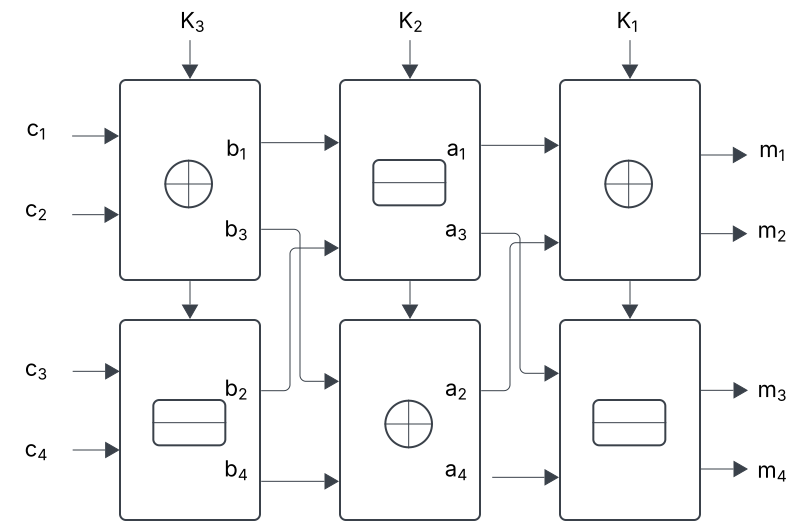
\includegraphics[scale=0.4]{aufgabe 2/img/decrypt.svg}
    \caption{Skizze der Entschlüsselung mit dem angegebenen Verfahren. (Quelle: eigene)}
    \label{fig:decrypt}
\end{figure}

\section{b)}

\textit{Bestimmen Sie das zum Klartext $m = ((1111),(0000),(1010),(0011))$ gehörende
Chiffrat $c = E_k (m)$, wobei $k = ((01001100),(00111111),(01101110))$ der verwendete
Schlüssel ist.
}\\

\noindent
Wir legen zunächst die Schlüsselkomponenten (\ref{eq:keycomp}) und Nachrichtenblöcke (\ref{eq:msgblock}) fest:

\begin{equation}\label{eq:keycomp}
\begin{split}
    k_{11} &= 0100\\
    k_{12} &= 1100\\
    k_{21} &= 0011\\
    k_{22} &= 1111\\
    k_{31} &= 0110\\
    k_{32} &= 1110
\end{split}
\end{equation}

\begin{equation}\label{eq:msgblock}
\begin{split}
    m_{1} &= 1111\\
    m_{2} &= 0000\\
    m_{3} &= 1010\\
    m_{4} &= 0011
\end{split}
\end{equation}

\vspace{5mm}

\noindent
Chiffrierte Blocktexte ermitteln:

\begin{equation}\notag
\begin{alignat}{3}
    a_1||a_2 &= (0100 \ 1100) \oplus (1111||0000) &&= (1011)||(1100)\\
    a_3||a_4 &= (0100 \boxminus 1010)||(1100 \boxminus 0011) &&= (1010)||(1001)\\
    b_1||b_2 &= (0011 \boxminus 1011)||(1111 \boxminus 1010) &&= (1000)||(0101)\\
    b_3||b_4 &= (0011 \ 1111) \oplus (1100||1001) &&= (1111)||(0110)
\end{alignat}
\end{equation}

\noindent
Wir erhalten:

\begin{equation}\notag
\begin{alignat}{3}
    c_1||c_2 &= (0110 \ 1110) \oplus (1000||1111) &&= (1110)||(0001)\\
    c_3||c_4 &= (0110 \boxminus 0101)||(1110 \boxminus 0110) &&= (0001)||(1000)
\end{alignat}
\end{equation}

\noindent
Insgesamt wird $m$ chiffriert zu

\begin{equation}\notag
E_k(m) =  E_k (1111\ 0000\ 1010\ 0011) = 1110 \ 0001 \ 0001 \ 1000
\end{equation}
